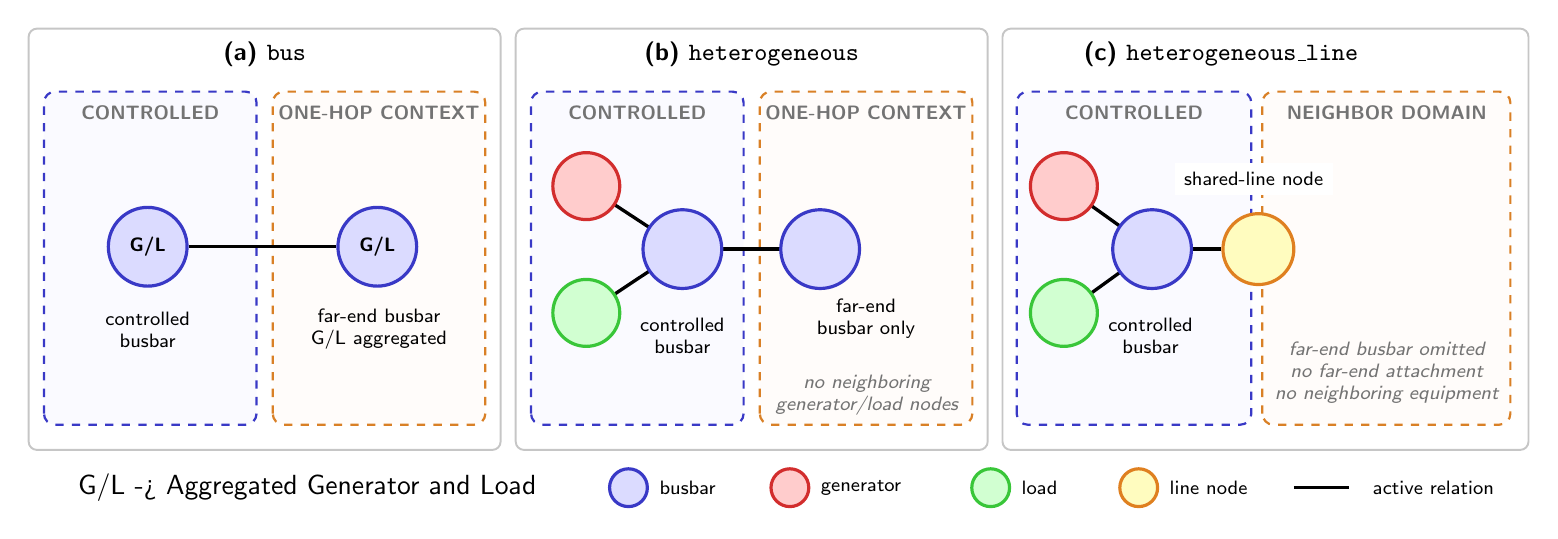
\begin{tikzpicture}[
  x=1cm,
  y=1cm,
  font=\sffamily,
  busbar/.style={
    circle,
    draw=blue!55!gray,
    fill=blue!14,
    line width=1.15pt,
    minimum size=10mm,
    inner sep=0pt
  },
  generator/.style={
    circle,
    draw=red!65!gray,
    fill=red!20,
    line width=1.15pt,
    minimum size=8.5mm,
    inner sep=0pt
  },
  load/.style={
    circle,
    draw=green!55!gray,
    fill=green!18,
    line width=1.15pt,
    minimum size=8.5mm,
    inner sep=0pt
  },
  linenode/.style={
    circle,
    draw=orange!75!gray,
    fill=yellow!25,
    line width=1.15pt,
    minimum size=9mm,
    inner sep=0pt
  },
  physical/.style={draw=black, line width=1.2pt},
  panel/.style={draw=gray!45, rounded corners=3pt, line width=0.7pt},
  controlled/.style={
    draw=blue!55!gray,
    dashed,
    rounded corners=4pt,
    fill=blue!2,
    line width=0.8pt
  },
  context/.style={
    draw=orange!70!gray,
    dashed,
    rounded corners=4pt,
    fill=orange!2,
    line width=0.8pt
  },
  zone/.style={font=\scriptsize\bfseries\sffamily, text=gray!75},
  label/.style={font=\scriptsize\sffamily, align=center},
  omitted/.style={font=\scriptsize\itshape\sffamily, align=center, text=gray!68}
]

% ---------------------------------------------------------------------------
% (a) Busbar representation
% ---------------------------------------------------------------------------
\begin{scope}[xshift=-19pt, xscale=1.08]
  \path[panel] (0,0) rectangle (5.55,5.35);
  \node[font=\bfseries\small\sffamily] at (2.775,5.02)
    {(a) \texttt{bus}};
  \path[controlled] (0.18,0.32) rectangle (2.68,4.55);
  \path[context] (2.87,0.32) rectangle (5.37,4.55);
  \node[zone, text=black!55] at (1.43,4.28) {CONTROLLED};
  \node[zone, text=black!55] at (4.12,4.28) {ONE-HOP CONTEXT};
  \node[busbar, font=\scriptsize\bfseries\sffamily] (bbus-c) at (1.4,2.58) {G/L};
  \draw[physical] (bbus-c.east) -- (3.61,2.58);
  \node[busbar, font=\scriptsize\bfseries\sffamily] (bbus-n) at (4.1,2.58) {G/L};
  \node[label] at (1.4,1.53) {controlled\\busbar};
  \node[label] at (4.12,1.53) {far-end busbar\\G/L aggregated};
\end{scope}

% ---------------------------------------------------------------------------
% (b) Disaggregated representation
% ---------------------------------------------------------------------------
\begin{scope}[xshift=157pt, xscale=1.08]
  \path[panel] (0,0) rectangle (5.55,5.35);
  \node[font=\bfseries\small\sffamily] at (2.775,5.02)
    {(b) \texttt{heterogeneous}};

  \path[controlled] (0.18,0.32) rectangle (2.68,4.55);
  \path[context] (2.87,0.32) rectangle (5.37,4.55);
  \node[zone, text=black!55] at (1.43,4.28) {CONTROLLED};
  \node[zone, text=black!55] at (4.12,4.28) {ONE-HOP CONTEXT};

  \draw[physical] (1.96,2.55) -- (3.58,2.55);
  \draw[physical] (0.83,3.35) -- (1.96,2.55);
  \draw[physical] (0.83,1.74) -- (1.96,2.55);

  \node[generator] (hgen) at (0.83,3.35) {};
  \node[load] (hload) at (0.83,1.74) {};
  \node[busbar] (hbus-c) at (1.96,2.55) {};
  \node[busbar] (hbus-n) at (3.58,2.55) {};

  \node[label] at (1.96,1.45) {controlled\\busbar};
  \node[label] at (4.12,1.67) {far-end\\busbar only};

  \node[omitted, text=black!55] at (4.13,0.70)
    {no neighboring\\generator/load nodes};
\end{scope}

% ---------------------------------------------------------------------------
% (c) Disaggregated representation with explicit line nodes
% ---------------------------------------------------------------------------
\begin{scope}[xshift=11.70cm]
  \path[panel] (0,0) rectangle (6.68,5.35);
  \node[font=\bfseries\small\sffamily] at (2.775,5.02)
    {(c) \texttt{heterogeneous\_line}};
  \path[controlled] (0.18,0.32) rectangle (3.16,4.55);
  \path[context] (3.3,0.32) rectangle (6.45,4.55);
  \node[zone, text=black!55] at (1.67,4.28) {CONTROLLED};
  \node[zone, text=black!55] at (4.88,4.28) {NEIGHBOR DOMAIN};
  \draw[physical] (1.90,2.55) -- (2.775,2.55);
  \draw[physical] (0.78,3.35) -- (1.90,2.55);
  \draw[physical] (0.78,1.74) -- (1.90,2.55);
  \node[generator] (lgen) at (0.78,3.35) {};
  \node[load] (lload) at (0.78,1.74) {};
  \node[busbar] (lbus-c) at (1.90,2.55) {};
  \node[linenode] (line) at (3.25,2.55) {};
  \node[label] at (1.88,1.45) {controlled\\busbar};
  \node[omitted, text=black!55] at (4.88,0.98)
    {far-end busbar omitted\\no far-end attachment\\no neighboring equipment};
  \node[label, fill=white] at (3.19,3.44) {shared-line node};
\end{scope}

% Compact shared legend.
\node[busbar, minimum size=4.8mm] at (6.95,-0.48) {};
\node[label, anchor=west] at (7.22,-0.48) {busbar};
\node[generator, minimum size=4.8mm] at (9,-0.48) {};
\node[label, anchor=west] at (9.27,-0.48) {generator};
\node[load, minimum size=4.8mm] at (11.55,-0.48) {};
\node[label, anchor=west] at (11.82,-0.48) {load};
\node[linenode, minimum size=4.8mm] at (13.43,-0.48) {};
\node[label, anchor=west] at (13.7,-0.48) {line node};
\draw[physical] (15.4,-0.48) -- (16.1,-0.48);
\node[label, anchor=west] at (16.28,-0.48) {active relation};

  \node[draw=none] at (2.87,-0.48) {G/L -> Aggregated Generator and Load};
\end{tikzpicture}
